\documentclass{mk-polish-lab-report}
%\linespread{1.05}
%\usepackage{lipsum}
%\usepackage[light, math]{anttor}
\usepackage{amsmath}
\usepackage{bm}
\usepackage{empheq}
\renewcommand{\arraystretch}{1,25}

\university{Politechnika Wrocławska}
\major{Informatyka, inż. I st.}
\tutor{dr hab. Paweł Zieliński}
\coursegroup{czwartek TN, 11:15}

\author{Miriam Jańczak}
\studentnumber{229761}
\title{Obliczenia naukowe}
\topic{Lista 5}


\usepackage{linegoal}
\usepackage{graphics}
\usepackage{tabularx}
\usepackage{pdflscape}
%\renewcommand{\thesubfigure}{\roman{subfigure}}
%\crefrangelabelformat{figure}{#3#1#4--#5#2#6}

\hyphenation{węz-łach}

%% Uncomment to change margins size
%\geometry{top=2.5cm,bottom=2cm,left=2.5cm,right=2.5cm}
%% Uncomment to change space between items
\setlist[enumerate]{itemsep=0pt}
\setlist[itemize]{itemsep=0pt}
\setlist[description]{itemsep=0pt}

\DeclareMathOperator{\sgn}{sgn}
\newcommand{\mA}{\bm{A}}
\newcommand{\mB}{\bm{B}}
\newcommand{\mC}{\bm{C}}
\newcommand{\mL}{\bm{L}}
\newcommand{\mU}{\bm{U}}
\newcommand{\mZ}{\bm{0}}
\newcommand{\vb}{\bm{b}}
\newcommand{\vx}{\bm{x}}
\newcommand{\R}{\mathbb{R}}

\begin{document}

\maketitle

\section{Opis problemu}

Rozwiązanie układu równań liniowych:
\begin{equation}
\mA\vx = \vb,
\label{eq:uklad}
\end{equation} 
dla danej macierzy $\mA \in \R^{n\times n}$ 
i wektora prawych stron $\vb \in \R^n$, gdzie $n \geq 4$. \\

\noindent Macierz $\mA$ jest rzadką macierzą blokową o następującej strukturze:
\begin{equation}
\mA =
\left(\begin{array}{ccccccc}
\mA_1 & \mC_1 & \mZ & \mZ & \mZ & \cdots & \mZ \\
\mB_2 & \mA_2 & \mC_2 & \mZ & \mZ  & \cdots & \mZ \\
\mZ  & \mB_3 & \mA_3 & \mC_3 & \mZ  & \cdots & \mZ \\
\vdots & \ddots & \ddots & \ddots & \ddots & \ddots & \vdots\\
\mZ   & \cdots & \mZ  & \mB_{v-2} & \mA_{v-2} & \mC_{v-2} & \mZ \\
\mZ  & \cdots & \mZ  &  \mZ &\mB_{v-1} & \mA_{v-1} & \mC_{v-1}  \\
\mZ  & \cdots & \mZ & \mZ & \mZ& \mB_{v} & \mA_{v}  \\
\end{array}\right),
\label{eq:postac}
\end{equation} 
$v = \frac{n}{\ell}$, zakładając że $n$ jest podzielne przez $\ell$, gdzie $\ell \geq 2$ jest rozmiarem wszystkich kwadratowych macierzy wewnętrznych (bloków) $\mA_i$, $\mB_i$, $\mC_i$, $\mZ$. \\

\noindent Macierze $\mA_i$, $\mB_i$, $\mC_i$, $\mZ$ są następującej postaci:
\begin{enumerate}[(i)]
\item $\mA_i \in \R^{\ell\times \ell}$,   $i = 1, \ldots,v$ -- macierze gęste,
\item $\mZ \in \R^{\ell\times \ell}$ -- macierz zerowa, 
\item $\mB_i \in \R^{\ell\times \ell}$,   $i = 2, \ldots,v$ -- macierze z niezerowymi dwoma ostatnimi kolumnami:
\begin{equation}
\mB_i =
\left(\begin{array}{ccccc}
0 & \cdots & 0 & b_{1\,\ell-1}^i & b_{1\,\ell}^i \\
0 & \cdots & 0 & b_{2\,\ell-1}^i & b_{2\,\ell}^i \\
\vdots & & \vdots & \vdots & \vdots \\
0 & \cdots & 0 & b_{\ell\,\ell-1}^i & b_{\ell\,\ell}^i \\
\end{array}\right),
\end{equation} 
\item $\mC_i \in \R^{\ell\times \ell}$,   $i = 1, \ldots,v\!-\!1$ -- macierze diagonalne:
\begin{equation}
\mC_i =
\left(\begin{array}{ccccc}
 c_{1}^i & 0 & 0 & \cdots & 0  \\
0 &  c_{2}^i &  0 & \cdots & 0  \\
\vdots &  \ddots &  \ddots & \ddots & \vdots  \\
0 & \cdots & 0 &  c_{\ell-1}^i & 0 \\
0 & \cdots & 0 &  0 & c_{\ell}^i \\
\end{array}\right).
\end{equation} 
\end{enumerate}

\noindent W celu rozwiązania układu równań liniowych $\mA\vx = \vb$ \eqref{eq:uklad} należało zastosować dwie metody:
\begin{enumerate}[(a)]
\item metodę eliminacji Gaussa w wersji bez wyboru elementu głównego oraz z częściowym wyborem elementu głównego,   
\item obliczyć rozkład~$\mL\mU$ macierzy $\mA$ w wersji bez wyboru elementu głównego oraz z częściowym wyborem elementu głównego, a następnie rozwiązać układ $\mL\mU\vx = \vb$.
\end{enumerate}

\section{Sposób przechowywania macierzy}
Macierz $\mA$ dana w zadaniu posiada tylko $(\ell + 3)n - 3 \ell$ elementów nie będących zerami -- $v \cdot \ell^2$~w~blokach $\mA_i$, $(v-1) \cdot 2\ell$ w blokach $\mB_i$ i $(v-1) \cdot\ell$ w blokach~$\mC_i$, co świadczy o tym, że $\mA$ jest macierzą rzadką. Przechowywanie macierzy $\mA$ w standardowy sposób (tablica dwuwymiarowa $n\times n$) byłoby więc dość nieefektywne. Aby temu zapobiec użyta została specjalna struktura do przechowywania macierzy rzadkich \texttt{SparseMatrixCSC} z języka \texttt{Julia}, w której macierze przechowywane są w skompresowanym porządku kolumnowym. W celu optymalizacji czasowej dostępu do elementów tak przechowywanej macierzy pod kątem zaimplementowanych algorytmów używano macierzy transponowanej, co jednak nie miało wpływu na ogólną ich postać, dlatego zostanie pominięte w rozważaniach.

\section{Opis algorytmów}
\emph{Metoda eliminacji Gaussa} jest algorytmem mającym szerokie zastosowanie w rozwiązywaniu podstawowych problemów algebry liniowej takich jak rozwiązywanie układów równań liniowych, obliczanie rzędu macierzy, jej wyznacznika, macierzy odwrotnej czy rozkładu $\mL\mU$ macierzy. Wykorzystuje ona elementarne operacje na macierzy takie jak mnożenie wiersza przez skalar czy odejmowanie od siebie dwóch wierszy.

\subsection{Rozwiązywanie układów równań metodą eliminacji Gaussa} 

\subsubsection{Opis działania}

Zasadą działania \emph{metody eliminacji Gaussa} przy rozwiązywaniu układów równań jest stopniowa eliminacja niewiadomych przez odpowiednie kombinowanie równań tak, aby zastąpić dany układ $\mA\vx = \vb$ równoważnym mu układem z macierzą trójkątną górną. \\
\noindent W pierwszym kroku zostaje wyeliminowana niewiadoma $x_{1}$ z $n-1$ równań poprzez odejmowanie dla $i = 2, \cdots, n$ odpowiedniej krotności pierwszego równania od $i$-tego równania, aby wyzerować w nim współczynnik przy $x_{1}$. Takie postępowanie powtarzane jest dla kolejnych niewiadomych $x_{k}$, gdzie dla $i = k+1, \cdots, n$ od $i$-tego równania odejmowana jest odpowiednia krotność $k$-tego równania. \\

\noindent Aby możliwe było wykonanie powyższej procedury każdy z elementów diagonalnych w macierzy musi być różny od zera. W momencie kiedy tak nie jest potrzebna jest modyfikacja algorytmu, a mianowicie zamiana wiersza z zerowym elementem na diagonali z innym który w tym miejscu nie posiada zera, w praktyce w $i$-tym kroku algorytmu wyszukuje się w $i$-tej kolumnie element (zwany \emph{elementem głównym}) o największej co do modułu wartości i wiersz z takim elementem zamienia się miejscem z $i$-tym wierszem. Taka zamiana zawsze jest możliwa, gdyż w przeciwnym przypadku macierz byłaby osobliwa. \\

\noindent Ostatnim krokiem jest rozwiązanie powstałego układu z macierzą trójkątną górna za pomocą \emph{algorytmu podstawiania wstecz}. Polega on na obliczeniu:

\begin{equation*}
x_i = \frac{b_i - \sum_{j = i+1}^n a_{ij}}{a_{ii}}
\end{equation*}
dla wierszy $i$ od $n$ do $1$.  \\

\noindent Metoda eliminacji Gaussa ma złożoność $O(n^3)$, a algorytm podstawiania wstecz $O(n^2)$. Zatem, aby rozwiązać układ równań, trzeba wykonać łącznie $O(n^3)$ operacji.

\subsubsection{Zastosowane modyfikacje}

Jak już zostało wspomniane, macierz $\mA$ jest macierzą rzadką ponadto posiada ona specyficzną blokowo-trójdiagonalną postać \eqref{eq:postac} co umożliwia zredukowanie w znacznym stopniu liczby wykonywanych operacji w stosunku do metody eliminacji Gaussa stosowanej dla macierzy gęstych. \\

\noindent Zauważyć można, że postać macierzy $\mA$ zapewnia, że wiele elementów znajdujących się pod diagonalą będzie zerami i nie będzie konieczne ich zerowanie. \\

\noindent Rozpatrując pierwszych $\ell-2$ kolumn widać że elementy niezerowe mogą znajdować się jedynie w bloku $\mA_1$, a więc tylko w $\ell$ pierwszych rzędach. Idąc dalej, dla kolejnych $\ell$ kolumn wszystkie niezerowe elementy będą znajdować się najniżej w bloku $\mB_2$ albo w bloku $\mA_3$ -- czyli $2\ell$ pierwszych rzędach, a dla jeszcze następnych $\ell$ kolumn w blokach $\mB_3$ i $\mA_4$ -- czyli $3\ell$ pierwszych rzędach. Biorąc pod uwagę następne kolumny schemat będzie się powtarzał dając możliwość wyprowadzenia ogólnego wzoru na indeks ostatniego niezerowego elementu $e_{non~0}$ w danej kolumnie $k$:

\begin{equation}
e_{non~0}(k) = \min\left\lbrace\ell + \ell \cdot \left \lfloor\frac{k + 1}{\ell}\right \rfloor, n\right\rbrace
\end{equation}

\noindent Również, poza ostatnimi $\ell$ wierszami, w każdym wierszu ostatnim niezerowym elementem jest element leżący na diagonali bloku $\mC_i$. Można zauważyć, że owe elementy znajdują się zawsze w odległości $\ell$ od elementów na diagonali macierzy $\mA$. Natomiast dla ostatnich $\ell$ rzędów najbardziej wysunięte na prawo elementy niezerowe leżą w $n$-tej kolumnie. Powyższa obserwacja pozwala na wyprowadzenie wzoru tym razem na indeks kolumny $k_{last}$, w której znajduje się ostatni niezerowy element w rzędzie $r$:

\begin{equation}
k_{last}(r) = \min\{r + \ell, n\}.
\label{eq:max_col}
\end{equation}

\noindent Oczywiście, jeżeli w danym kroku metody eliminacji Gaussa $r$-ty rząd odejmowany jest od rzędów pod nim, nie jest konieczne modyfikowanie elementów w kolumnach o większych od $k_{last}(r)$ indeksach. \\

\noindent Metoda eliminacji Gaussa prowadzi do układu z macierzą trójkątną górną, który rozwiązywany jest za pomocą algorytmu podstawiania wstecz, który w tym przypadku także poddawany jest drobnym modyfikacjom w celu ograniczenia liczby wykonywanych operacji. \\

\noindent Warto zauważyć tutaj, że w wyniku eliminacji Gaussa poza elementami pod diagonalą bloków $\mC_i$ w macierzy $\mA$ nie powstały żadne nowe elementy niezerowe. Wystarczy zatem dla każdego wiersza sumować elementy tylko do pewnej kolumny określonej wyprowadzonym wcześniej wzorem \eqref{eq:max_col}. \\

\noindent Metodę eliminacji Gaussa z opisanymi modyfikacjami przedstawia \Cref{alg:gauss}. \\

\noindent Zakładając, że $\ell$ jest stałą, złożoność obliczeniowa zmodyfikowanej metody eliminacji Gaussa, wynosi $O(n)$. Zewnętrzna pętla eliminacji Gaussa wykonuje $n-1$ przebiegów, środkowa maksymalnie $2\ell$, natomiast wewnętrzna maksymalnie $\ell$. Z kolei w algorytmie podstawiania wstecz zewnętrzna pętla wykonuje $n$ przebiegów, natomiast wewnętrzna maksymalnie $\ell$. Jest to znacząca poprawa względem standardowej metody eliminacji Gaussa.

\begin{algorithm}[h]
%			\LinesNumbered
    			\SetKwInOut{Input}{Dane wejściowe}
    			\SetKwInOut{Output}{Dane wyjściowe}
    			\SetKwProg{Fn}{function}{}{}
    			\SetKw{KwDownTo}{downto}
    			\SetKw{Err}{error}
    			
			\SetKwData{L}{$\ell$} 			
			\SetKwData{N}{$n$}    				
			\SetKwData{B}{$\vb$}    		
			\SetKwData{A}{$\mA$}    			
    			\SetKwData{X}{$\vx$}
    			\SetKwData{F}{f}
    			\SetKwData{Z}{z}
    			\SetKwData{I}{i}
    			\SetKwData{J}{j}
    			\SetKwData{K}{k}
    			\SetKwData{Sum}{suma}
    			\SetKwData{Col}{$k_{last}$}
    			\SetKwData{Row}{$e_{non~0}$}
			\SetKwFunction{ge}{eliminacja\_gaussa}
			\SetKwFunction{Min}{$\min$}

		    \Input{\\
	    \begin{tabularx}{0.85\linewidth}{rcX}
  			{\A} & -- & dana w zadaniu macierz postaci \eqref{eq:postac},\\
  			{\B} & -- & wektor prawych stron, \\
  			{\N} & -- & rozmiar macierzy \A, \\
  			{\L} & -- & rozmiar bloku macierzy \A.  		
		\end{tabularx}
			}
		    \Output{\\
		    \begin{tabularx}{0.85\linewidth}{rcX}
    			{\X}& -- & wektor zawierający rozwiązania układu $\A\X=\B$.
			\end{tabularx}					    			
		    	}
		    	\Fn{\ge{\A,~\B,~\N,~\L}}{
		    		\For{$\K \gets 1$ \KwTo $\N-1$} {
		    		$\Row\gets\Min\left(\L + \L \cdot \left \lfloor\frac{\K + 1}{\ell}\right \rfloor, n\right)$\;
		    		$\Col\gets \Min(\K + \L, \N)$\;
		    		\For{$\I \gets \K+1$ \KwTo \Row}{
		    			\If{$\A[\K][\K] = 0$}{\Err współczynnik na przekątnej równy zeru}
		    			$\Z \gets \A[\I][\K] / \A[\K][\K]$\;
		    			$\A[\I][\K] \gets 0 $ \;
		    			\For{$\J \gets \K+1$ \KwTo \Col}{
		    				$\A[\I][\J] \gets \A[\I][\J] - \Z \cdot \A[\K][\J]$\;
		    			}
		    			$\B[\I] \gets \B[\I] - \Z \cdot \B[\K]$\;
		    		}
		    		}
		   \For{$\I \gets \N$ \KwDownTo $1$}{
		   		$\Col\gets \Min(\I+ \L, \N)$\;
		   		\For{$\J \gets \K+1$ \KwTo $\Col$}{
				$\Sum \gets \Sum + \X[\I] \cdot \A[\I][\J]$\;
		   		}
		   		$\X[\I] \gets (\B[\I] - \Sum) / \A[\I][\I]$\;
		   }
		   		   
    			\KwRet \X\;
			}
\caption{Eliminacja Gaussa}\label{alg:gauss}
\end{algorithm} 

\noindent Powyżej został rozpatrzony wariant metody eliminacji Gaussa bez wyboru elementu głównego, czasami jednak lepiej sprawdza się algorytm z tzw. częściowym wyborem (umożliwia rozwiązanie układu kiedy na diagonali macierzy pojawiają się elementy zerowe), w tym wypadku oznacza to wybranie wiersza, dla którego element w eliminowanej kolumnie $i$ ma największą co do modułu wartość i zamienienie go z $i$-tym wierszem (po zamianie eliminacja jest kontynuowana w zwykły sposób). \\

\noindent W praktyce taka zamiana wierszy bywa kosztowna, szczególnie kiedy operacje wykonywane są na dużych macierzach, dlatego przy metodzie eliminacji Gaussa z wyborem elementu głównego pierwszą wprowadzoną zmianą jest stworzenie wektora permutacji wierszy ($p$), w którym pamiętane jest na jakiej aktualnie pozycji w macierzy znajduje się dany wiersz. Wpływ tego zabiegu na algorytm jest taki, że zamiast odwołania do konkretnego wiersza zostaje wykonane odwołanie do jego pozycji w wektorze permutacji. \\

\noindent Wybór elementu głównego sprawia również, że niemożliwe jest zachowanie wyliczonych wartości $k_{last}$, gdyż odejmowanie wierszy w innej kolejności, może doprowadzić do powstania nowych elementów niezerowych. Konieczne jest zatem nowe, szersze oszacowanie $k_{last}$. Zauważyć można, że w czasie eliminowania współczynników z $\ell - 2$ pierwszych kolumn najdalszy niezerowy element można stworzyć w kolumnie z indeksem $2\ell$ -- poprzez odejmowanie $\ell$-tego wiersza, który w tej kolumnie posiada niezerowy element. Podczas eliminowania współczynników z kolejnych $\ell$ kolumn  najdalszy niezerowy element można stworzyć w kolumnie z indeksem $3\ell$, analogicznie poprzez odejmowanie $2\ell$-tego wiersza, który w tej kolumnie posiada niezerowy element. Stosowanie powyższego rozumowania dla dalszych kolumn prowadzi do uzyskania nowego wzoru na $k_{last}$, mianowicie:  

\begin{equation}
k_{last}(k) = \min\left\lbrace2\ell + \ell \cdot \left \lfloor\frac{k + 1}{\ell}\right \rfloor, n\right\rbrace.
\label{eq:max_col_piv}
\end{equation}

\noindent Podobne ograniczenie zastosowane jest również podczas wykonywania algorytmu podstawiania wstecz -- nie powstają żadne nowe elementy niezerowe poza tymi już uwzględnionymi, jedyną zmianą jest uwzględnienie permutacji wiersza, co jednak w zasadzie nie wpływa na szacowaną wartość. \\

\noindent Metodę eliminacji Gaussa z częściowym wyborem elementu głównego przedstawia \Cref{alg:pivotgauss} \\

\noindent Złożoność obliczeniowa zmodyfikowanej metody eliminacji Gaussa z częściowym wyborem elementu głównego jest gorsza niż bez wyboru elementu głównego z powodu zastosowanych szerszych ograniczeń na $k_{last}$, jednak przy założeniu, że $\ell$ jest stałą nie wpływa to na ogólną złożoność $O(n)$.

\begin{algorithm}[h]
    			\SetKwInOut{Input}{Dane wejściowe}
    			\SetKwInOut{Output}{Dane wyjściowe}
    			\SetKwProg{Fn}{function}{}{}
    			\SetKw{KwDownTo}{downto}
    			\SetKw{Err}{error}
    			
			\SetKwData{L}{$\ell$} 			
			\SetKwData{N}{$n$}    				
			\SetKwData{B}{$\vb$}    		
			\SetKwData{A}{$\mA$}    			
    			\SetKwData{X}{$\vx$}
    			\SetKwData{F}{f}
    			\SetKwData{Z}{z}
    			\SetKwData{I}{i}
    			\SetKwData{J}{j}
    			\SetKwData{K}{k}
    			\SetKwData{Mm}{m}
   			\SetKwData{P}{p}
   			\SetKwData{Q}{q}
    			\SetKwData{Sum}{suma}
    			\SetKwData{Idx}{$r_{\max}$}
    			\SetKwData{Val}{$v_{\max}$}
    			\SetKwData{Col}{$k_{last}$}
    			\SetKwData{Row}{$e_{non~0}$}
			\SetKwFunction{ge}{eliminacja\_gaussa\_z\_elementem\_głównym}
			\SetKwFunction{Min}{$\min$}
			\SetKwFunction{Swap}{swap}

		    \Input{\\
	    \begin{tabularx}{0.85\linewidth}{rcX}
  			{\A} & -- & dana w zadaniu macierz postaci \eqref{eq:postac},\\
  			{\B} & -- & wektor prawych stron. \\
  			{\N} & -- & rozmiar macierzy \A, \\
  			{\L} & -- & rozmiar bloku macierzy \A.  		
		\end{tabularx}
			}
		    \Output{\\
		    \begin{tabularx}{0.85\linewidth}{rcX}
    			{\X}& ---& wektor zawierający rozwiązania układu $\A\X=\B$.
			\end{tabularx}		    			
		    	}
		    	\Fn{\ge{\A,~\B,~\N,~\L}}{
		    		$\P \gets \{\I : \I \in \{1, \ldots, n \} \}$\;
		    		\For{$\K \gets 1$ \KwTo $\N-1$} {
		    		$\Row\gets\Min\left(\L + \L \cdot \left \lfloor\frac{\K + 1}{\ell}\right \rfloor\!, n\right)$\;
		    		$\Col\gets \Min\left(2\L + \L \cdot \left \lfloor\frac{\K + 1}{\ell}\right \rfloor\!, \N\right)$\;
		    		\For{$\I \gets \K+1$ \KwTo \Row}{
		    			$\Idx \gets \Mm$ takie, że: $\A[\P[\Mm]][\K] = \max(|\A[\P[\Q]][\K]| : \Q \in \{\I, \ldots,\Row\} )$\;
		 		
		    			\If{$\P[\Idx] = 0$}{\Err macierz osobliwa}
		    			\Swap($\P[\K], \P[\Idx]$)\;
		    			$\Z \gets \A[\P[\I]][\K] / \A[\P[\K]][\K]$\;
		    			$\A[\P[\I]][\K] \gets 0 $ \;
		    			\For{$\J \gets \K+1$ \KwTo \Col}{
		    				$\A[\P[\I]][\J] \gets \A[\P[\I]][\J] - \Z \cdot \A[\P[\K]][\J]$\;
		    			}
		    			$\B[\P[\I]] \gets \B[\P[\I]] - \Z \cdot \B[\P[\K]]$\;
		    		}
		    		}
		   \For{$\I \gets \N$ \KwDownTo $1$}{
		   		$\Col\gets \Min\left(2\L + \L \cdot \left \lfloor\frac{\P[\I] + 1}{\ell}\right \rfloor\!, \N\right)$\;
		   		\For{$\J \gets \K+1$ \KwTo $\Col$}{
				$\Sum \gets \Sum + \X[\J] \cdot \A[\P[\I]][\J]$\;
		   		}
		   		$\X[\I] \gets (\B[\P[\I]] - \Sum) / \A[\P[\I]][\I]$\;
		   }
		   		   
    			\KwRet \X\;
			}
\caption{Eliminacja Gaussa z częściowym wyborem elementu głównego}\label{alg:pivotgauss}
\end{algorithm} 

\subsection{Rozkład LU}

\subsubsection{Opis działania}

Układy równań liniowych z niektórymi typami macierzy da się rozwiązać w sposób stosunkowo łatwy, takimi macierzami są np. macierze trójkątne -- górna i dolna. Idea rozkładu $\bm{LU}$ macierzy $\mA$ jest taka, żeby przedstawić ją za pomocą iloczynu
\begin{equation}
\mA = \mL\mU,
\end{equation}
macierzy trójkątnej dolnej $\mL$ z elementami na przekątnej równymi $1$ i macierzy trójkątnej górnej $\mU$, za pomocą których układ równań da się rozwiązać w stosunkowo łatwy sposób. \\

\noindent Taki rozkład można uzyskać za pomocą znanej już metody eliminacji Gaussa. Metoda ta przekształca macierz $\mA$ do macierzy trójkątnej górnej, która stanie się macierzą $\mU$. Macierz $\mL$ zostaje stworzona poprzez zapamiętanie mnożników użytych do eliminacji kolejnych współczynników macierzy $\mA$ i tak mnożnik użyty do wyzerowania elementu $a_{ij}$ zapisujemy w $i$-tym wierszu i $j$-tej kolumnie macierzy $\mL$. Cały rozkład $\mL\mU$ można przeprowadzić bezpośrednio na macierzy $\mA$ oszczędzając w ten sposób pamięć. \\

\noindent Złożoność obliczeniowa wyznaczenia rozkładu $\mL\mU$ to $O(n^3)$, umożliwia on jednak stosunkowo szybkie rozwiązywanie wielu układów równań w których macierz jest taka sama, a zmienia się wektor prawych stron. W tym wypadku eliminacja Gaussa o dużej złożoności wykonywana jest tylko raz, a rozwiązywanie układów dzieli się na dwa etapy:
\begin{empheq}[left = \empheqlbrace]{align}
\mL \bm{z} &= \vb \nonumber\\
\mU \vx &= \bm{z},
\label{eq:etapy}
\end{empheq}
co dzięki postaci macierzy $\mL$ i $\mU$ (macierze trójkątne) można wykonać w $O(n^2)$ operacji.

\subsubsection{Zastosowane modyfikacje}

Rozkład $\bm{LU}$ dla macierzy $\mA$ w postaci (\ref{eq:postac}) jest wyznaczany w sposób bardzo podobny do metody eliminacji Gaussa (bez wyboru elementu głównego bądź z częściowym jego wyborem). Jednak zamiast zerowania elementów $a_{ik}$ podstawiane są mnożniki $z = {a_{ik}}/ {a_{kk}}$, które stanowią elementy macierzy $\mL$. \\

\noindent Złożoność obliczeniowa wyznaczenia takiego rozkładu jest w oczywisty sposób taka sama, co złożoność dla metody eliminacji Gaussa bez wyboru elementu głównego (\Cref{alg:gauss}) czy z częściowym jego wyborem (\Cref{alg:pivotgauss}), a więc, przy założeniu, że $\ell$ jest stałą, wynosi $O(n)$. \\

\noindent W celu rozwiązania układu równań liniowych $\mA\vx = \vb$, gdzie $\mA = \mL\mU$ czyli $\mL\mU\vx = \vb$ należy podzielić obliczenia na dwa etapy (\ref{eq:etapy}). Drugi etap obliczeń czyli rozwiązanie układu $\mU \vx = \bm{z}$ nie różni się w zasadzie niczym od algorytmu podstawiania wstecz, nie ulega także zmianie wartość $k_{last}$, która wskazuje na to do której kolumny w danym wierszy należy sumować. Aby rozwiązać układ $\mL \bm{z} = \vb$ należy zastosować algorytm podstawiania w przód, który jest podobny do algorytmu podstawiania wstecz, jednak zaczyna się od pierwszego wiersza i sumowane są elementy z kolumn coraz dalszych, a nie coraz wcześniejszych. Algorytm obliczania $\mL \bm{z} = \vb$ został oczywiście odpowiednio zoptymalizowany ze względu na specyficzną postać macierzy. Warto zauważyć że elementy zerowe w macierzy $\mL$ są na tych samych indeksach co te w macierzy $\mA$. Niepotrzebne jest więc rozpoczynanie sumowania od pierwszej kolumny dla każdego wiersza. W zasadzie takie sumowanie ma miejsce tylko dla $\ell$ pierwszych wierszy. Dla kolejnych $\ell$ wystarczy sumować od kolumny $\ell-1$, a dla jeszcze dalszych $\ell$ kolumny $2\ell-1$, itd. Tę zależność można przedstawić za pomocą następującego ogólnego wzoru:
\begin{equation}
k_{from}(r) = \max\left\lbrace\ell \cdot \left \lfloor\frac{r - 1}{\ell}\right \rfloor - 1, 1 \right\rbrace.
\end{equation}

\noindent Metodę rozwiązania układu równań liniowych za pomocą rozkładu $\mL\mU$ macierzy $\mA$ prezentuje \Cref{alg:LU-sol}. Metoda wykorzystująca rozkład $\mL\mU$ za pomocą eliminacji Gaussa z częściowym wyborem elementu głównego jest niemalże identyczny z tą tylko różnicą że zamiast odwołania się do konkretnego wiersza następuje odwołanie do jego pozycji w wektorze permutacji.\\ 

\noindent Złożoność obliczeniowa rozwiązywania układu równań liniowych z rozkładu $\mL\mU$ wynosi $O(n)$, ponieważ rozwiązanie $\mU \vx = \bm{z}$ ma taką samą złożoność jak w metodzie Gaussa, a  rozwiązanie $\mL \bm{z} = \vb$ w oczywisty sposób ma także zbliżoną do tej złożoność.

\begin{algorithm}[h]
    			\SetKwInOut{Input}{Dane wejściowe}
    			\SetKwInOut{Output}{Dane wyjściowe}
    			\SetKwProg{Fn}{function}{}{}
    			\SetKw{KwDownTo}{downto}
    			\SetKw{Err}{error}
    			
			\SetKwData{L}{$\ell$} 			
			\SetKwData{N}{$n$}    				
			\SetKwData{B}{$\vb$}    		
			\SetKwData{A}{$\mA$}    			
    			\SetKwData{X}{$\vx$}
    			\SetKwData{F}{f}
    			\SetKwData{Z}{z}
    			\SetKwData{I}{i}
    			\SetKwData{J}{j}
    			\SetKwData{K}{k}
    			\SetKwData{Sum}{suma}
    			\SetKwData{Col}{$k_{last}$}
    			\SetKwData{Colmin}{$k_{from}$}
			\SetKwFunction{ge}{rozwiązanie\_LU}
			\SetKwFunction{Min}{$\min$}

		    \Input{\\
	    \begin{tabularx}{0.85\linewidth}{rcX}
  			{\A} & -- & macierz \eqref{eq:postac} po przekształceniu do postaci, gdzie nad przekątną znajdują się elementy macierzy $\mU$, a pod przekątną $\mL$,\\
  			{\B} & -- & wektor prawych stron. \\
  			{\N} & -- & rozmiar macierzy \A, \\
  			{\L} & -- & rozmiar bloku macierzy \A.  		
		\end{tabularx}
			}
		    \Output{\\
		    \begin{tabularx}{0.85\linewidth}{rcX}
    			{\X}& -- & wektor zawierający rozwiązania układu $\A\X=\B$.
			\end{tabularx}		    			
		    	}
		    	\Fn{\ge{\A,~\B,~\N,~\L}}{
		    		\For{$\I \gets 1$ \KwTo $\N$} {
		    		$\Sum \gets 0$\;
		    		$\Colmin\gets \Min\left(\L \cdot \left \lfloor\frac{\I - 1}{\ell}\right \rfloor, n\right)$\;
		    		\For{$\J \gets \Colmin\;$\KwTo $\I - 1$}{
		    			$\Sum \gets \Sum + \Z[\J] \cdot \A[\I][\J]$\;
		    		}
		    		$\Z[\I] = \B[\I] - \Sum$\; 
		    		}
		   \For{$\I \gets \N$ \KwDownTo $1$}{
		   		$\Sum \gets 0$\;
		   		$\Col\gets \Min(\I+ \L, \N)$\;
		   		\For{$\J \gets \I+1$ \KwTo $\Col$}{
				$\Sum \gets \Sum + \X[\J] \cdot \A[\I][\J]$\;
		   		}
		   		$\X[\I] \gets (\Z[\I] - \Sum) / \A[\I][\I]$\;
		   }
		   		   
    			\KwRet \X\;
			}
\caption{Rozwiązywanie układu równań przy użyciu rozkładu $\mL\mU$.}\label{alg:LU-sol}
\end{algorithm} 

\subsection{Wyniki}
Zestawienie czasu rozwiązywania układów równań oraz zużytej pamięci, dla coraz większych macierzy $\mA$ standardową metodą eliminacji Gaussa jak również dwoma modyfikacjami -- bez wyboru elementu głównego i jego częściowym wyborem przedstawia \Cref{table:1}, dla metody bez modyfikacji obliczenia przerwano po rozwiązaniu układu z $6000$ niewiadomych, ponieważ zbyt duże zużycie pamięci uniemożliwiało dalszą pracę komputera. We wszystkich przedstawianych wynikach przyjęto rozmiar bloku $\ell = 4$.

\begin{table}[!h]
        \centering
        \footnotesize
\begin{tabular}{c
		|S[
        table-number-alignment = right,
		table-figures-integer  = 2,
		table-figures-decimal = 6
		]
		|c|S[
        table-number-alignment = right,
		table-figures-integer  = 2,
		table-figures-decimal = 6
		]
		|c|S[
        table-number-alignment = right,
		table-figures-integer  = 2,
		table-figures-decimal = 6
		]
		|c}
& \multicolumn{2}{c|}{$\vx = \mA \backslash \vb$} & \multicolumn{2}{c|}{bez wyboru} & \multicolumn{2}{c}{z wyborem} \\ \hline
$n$ & {Czas [s]} & {Pamięć} & {Czas [s]} & {Pamięć} & {Czas [s]} & {Pamięć} \\ \hline
16 & 0.001094 & 2.625 KiB & 0.000048 & 3.391 KiB & 0.000084 & 3.625 KiB \\
100 & 0.027763 & 80.047 KiB & 0.000179 & 22.500 KiB & 0.000407 & 23.406 KiB \\
2000 & 0.343397 & 30.549 MiB & 0.014192 & 453.000 KiB & 0.014862 & 468.781 KiB \\
6000 & 6.731499 & 274.750 MiB & 0.128058 & 1.327 MiB & 0.130757 & 1.373 MiB \\
10000 & {---} & --- & 0.381457 & 2.212 MiB & 0.384041 & 2.289 MiB \\
50000 & {---} & --- & 17.542994 & 5.722 MiB & 20.042335 & 6.104 MiB \\
\end{tabular}
\caption{Zestawienie czasu wykonywania i zużytej pamięci dla metody eliminacji Gaussa bez modyfikacji i metod z modyfikacjami w wariancie bez wyboru elementu głównego i z jego częściowym wyborem}
\label{table:1}
\end{table}	

\noindent Dla wspomnianych wcześniej metod zbadano również błędy, kiedy wektor prawych stron był wyliczany, przedstawia je \Cref{table:2}. Widać tutaj, że błędy wynikające ze stosowania metody eliminacji Gaussa z częściowym wyborem elementu głównego są mniejsze od tych powstałych przy rozwiązywaniu układu równań metodą bez wyboru elementu głównego o co najmniej rząd wielkości. Taka prawidłowość zachodzi również przy rozwiązywaniu układu równań za pomocą rozkładu $\mL\mU$ dlatego przedstawienie danych zostanie tutaj pominięte.

\begin{table}[!h]
        \centering
        \footnotesize
\begin{tabular}{c|
		S[
        table-number-alignment = right,
		table-figures-integer  = 1,
		table-figures-decimal = 16,
		table-figures-exponent = 3
		]
		|S[
        table-number-alignment = right,
		table-figures-integer  = 1,
		table-figures-decimal = 16,
		table-figures-exponent = 3
		]
		|S[
        table-number-alignment = right,
		table-figures-integer  = 1,
		table-figures-decimal = 16,
		table-figures-exponent = 3
		]
		}
$n$ & {$\vx = \mA \backslash \vb$} & {bez wyboru} & {z wyborem} \\ \hline
16 & 1.942890293094024e-16 & 3.107895799689565e-14 & 3.433175098891678e-16 \\
100 & 2.8522145930998397e-16 & 2.949121011348651e-15 & 2.6107951392584033e-16 \\
2000 & 2.7128998740608095e-16 & 2.9256114662419202e-15 & 3.0136983042333716e-16 \\
6000 & 2.9024777490400715e-16 & 1.96505177640419e-14 & 3.000171026473022e-16 \\
10000 & {---} & 4.459026580959929e-14 & 2.98232852765259e-16 \\
50000 & {---} & 4.503491569922606e-14 & 3.005195520712902e-16 \\
\end{tabular}
\caption{Zestawienie błędów względnych dla metody eliminacji Gaussa bez modyfikacji i metod z modyfikacjami w wariancie bez wyboru elementu głównego i z jego częściowym wyborem}
\label{table:2}
\end{table}	

\noindent Podobnie jak dla metody eliminacji Gaussa czas rozwiązywania układu oraz zużytą pamięć zbadano dla rozwiązywania z układem $\mL\mU$, z tym że osobno policzono czas i zużytą pamięć samego rozkładu, a następnie rozwiązania z użyciem tego rozkładu. W ten sposób można zaobserwować, że samo rozwiązanie z posiadanego rozkładu $\mL\mU$ jest ułamkiem nakładu czasu i pamięci potrzebnej do stworzenia rozkładu. Wyniki prezentuje \Cref{table:3}

\begin{table}[!h]
        \centering
        \footnotesize
\begin{tabular}{c
		|S[
        table-number-alignment = right,
		table-figures-integer  = 2,
		table-figures-decimal = 6
		]
		|c|S[
        table-number-alignment = right,
		table-figures-integer  = 2,
		table-figures-decimal = 6
		]
		|c|S[
        table-number-alignment = right,
		table-figures-integer  = 2,
		table-figures-decimal = 6
		]
		|c|S[
        table-number-alignment = right,
		table-figures-integer  = 2,
		table-figures-decimal = 6
		]
		|c}
& \multicolumn{2}{c|}{rozkład bez wyboru} & \multicolumn{2}{c|}{rozwiązanie bez wyboru} & \multicolumn{2}{c|}{rozkład z wyborem} & \multicolumn{2}{c}{rozwiązanie z wyborem} \\ \hline
$n$ & {Czas [s]} & {Pamięć} & {Czas [s]} & {Pamięć} & {Czas [s]} & {Pamięć} & {Czas [s]} & {Pamięć} \\ \hline
16 & 0.000035 & 3.188 KiB & 0.000006 & 416 b & 0.000073 & 3.422 KiB & 0.000012 & 416 b \\
100 & 0.000162 & 21.625 KiB & 0.000028 & 1.750 KiB & 0.000339 & 22.531 KiB & 0.000043 & 1.750 KiB \\
2000 & 0.011805 & 437.250 KiB & 0.000502 & 31.500 KiB & 0.014052 & 453.031 KiB & 0.000609 & 31.500 KiB \\
6000 & 0.118416 & 1.281 MiB & 0.001244 & 93.906 KiB & 0.129308 & 1.327 MiB & 0.002653 & 93.906 KiB \\
10000 & 0.376795 & 2.136 MiB & 0.002829 & 156.406 KiB & 0.381735 & 2.212 MiB & 0.003327 &  156.406 KiB \\
50000 & 17.361661 & 6.121 MiB & 0.055568 & 1.138 MiB & 18.941635 & 6.399 MiB & 0.074308 & 1.216 MiB \\
\end{tabular}
\caption{Zestawienie czasu wykonywania i zużytej pamięci dla rozkładów $\mL\mU$ w wariancie bez wyboru elementu głównego i z jego częściowym wyborem}
\label{table:3}
\end{table}

\noindent W celu potwierdzenia, że złożoność zmodyfikowanych metod jest rzeczywiście liniowa policzono liczbę operacji dla każdej z nich dla coraz większych macierzy, wyniki prezentuje \Cref{fig:wykres}.

\begin{figure}[h]
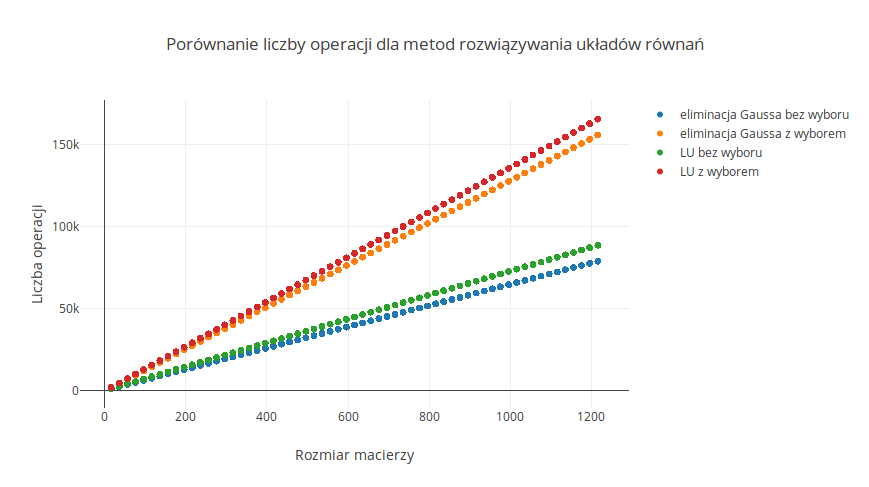
\includegraphics[width=\textwidth]{wykres.png}
\caption{Liczba operacji wykonywanych w czasie rozwiązywania układu równań poszczególnymi metodami}
\label{fig:wykres}
\end{figure} 	

\subsection{Wnioski}

Przedstawione wyniki pokazują, że rzeczywiście złożoność obliczeniowa zaimplementowanych metod jest liniowa. Widać także, że wolniejsza i zużywająca większą ilość pamięci metoda eliminacji z częściowym wyborem elementu głównego zarówno w metodzie eliminacji Gaussa jak i w rozkładzie $\mL\mU$ daje dokładniejsze wyniki, kiedy nieznacznie zostanie zaburzony wektor prawych stron. Warto pamiętać, że czasem jej użycie jest konieczne do rozwiązania układu (elementy zerowe na diagonali). Rozwiązywanie pojedynczych układów równań liniowych za pomocą rozkładu $\mL\mU$ jest sumarycznie gorsze od zastosowania metody eliminacji Gaussa, jednak kiedy dla jednej macierzy pojawia się więcej różnych wektorów prawych stron ta metoda staje się bardzo opłacalna, ponieważ sam rozkład macierzy jest liczony tylko raz, a rozwiązanie układu z dwóch macierzy trójkątnych jest szybsze i łatwiejsze niż przeprowadzenie eliminacji Gaussa od początku. Przeprowadzone eksperymenty pokazują również, że optymalizacja pod kątem specyficznej budowy macierzy $\mA$ daje konkretne rezultaty. Dzięki wprowadzonym modyfikacjom złożoność zarówno obliczeniowa jak i pamięciowa są na tyle małe że pozwalają na rozwiązywanie układów równań z bardzo dużą liczbą niewiadomych, co przy wykorzystaniu standardowych metod byłoby niemożliwe. Widać zatem jak wiele można zyskać optymalizując różne algorytmy pod konkretne przypadki użycia.

\end{document}
